% Author        : PokMan Ho pok.ho19@imperial.ac.uk
% Script        : model_01.tex
% Desc          : find candidates in model
% Input         : none
% Output        : pdf report in same directory
% Arguments     : 0
% Date          : Feb 2020

\documentclass[a4paper,11pt]{article}
\usepackage[margin=2cm]{geometry}
\usepackage[english]{babel}
\usepackage{graphicx, longtable, amsmath, amssymb, csquotes}
\graphicspath{{graph/}{graph/}}

\usepackage{xcolor,colortbl}
\definecolor{green}{rgb}{0,.4,0}

\usepackage{hyperref}
\hypersetup{
	colorlinks=true,
	linkcolor=green,
	filecolor=red,      
	urlcolor=blue,
	citecolor=orange
}

%% citation
\usepackage[%
autocite 	= superscript,
backend 	= bibtex,
sortcites 	= true,
style 		= nature
]{biblatex}
\bibliography{model_01.bib}

\title{Eco-Bioelectric Cell model idea}
\author{PokMan Ho}
\date{13 Feb 2020}

\begin{document}
    \maketitle
    \tableofcontents
    
    \section{aim}
    \begin{enumerate}
        \item find a suitable autotroph-heterotroph model to implement into this situation
        \item figure out meanings of each term in the candidate model(s)
    \end{enumerate}
    \section{Conceptual ebc}
    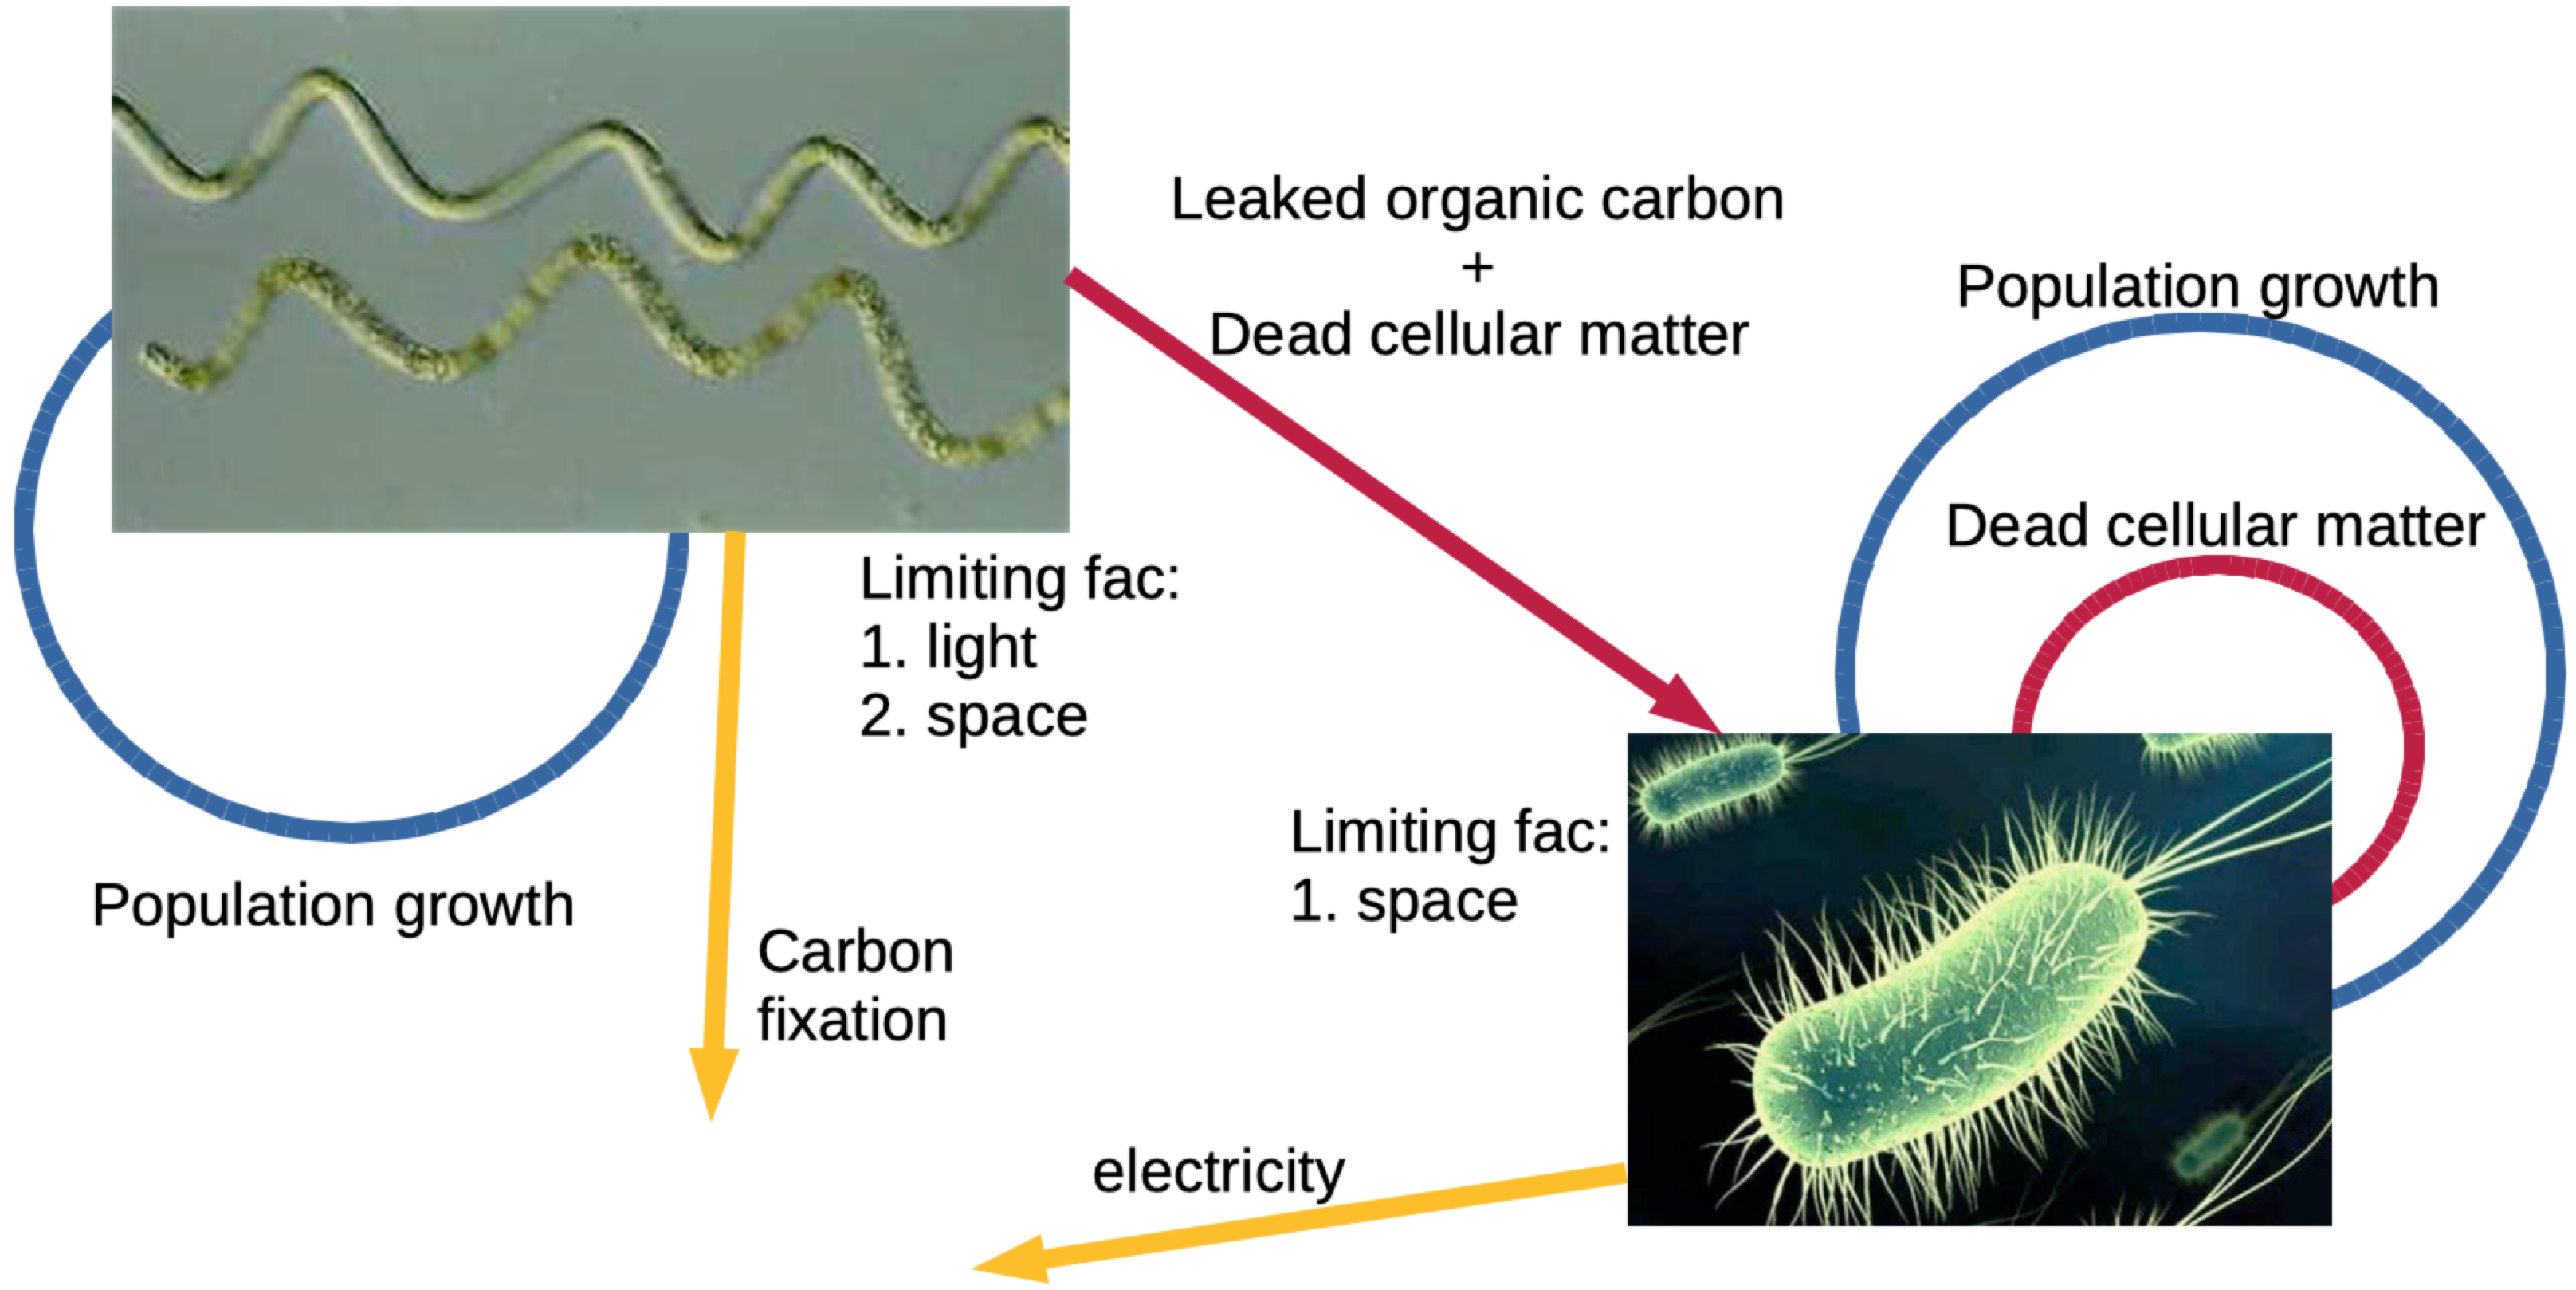
\includegraphics[width=\linewidth]{sandbox/graph/model_01.png}
    \section{what do i need}
    \begin{itemize}
        \item a one-/two-slab model for water column with benthic layer
        \item unlimited all-rounded nutrient supply
        \item NPD model (nutrient, phytoplankton, detritivore)
        \item no metabolites needed to be taken into account
        \item space limited
        \item address irradiation cycle
        \item address thermal performance fluctuation
    \end{itemize}
    \section{available NPZD models' features}
    \begin{enumerate}
        \item EMPOWER-1.0\autocite{anderson2015empower}
        \begin{itemize}
            \item seasonally varying surface mixed layer that contains the ecosystem positioned above a deep homogeneous layer containing unchanging nutrient and no plankton
            \item temperature dependencies for the physiological rates
            \item seasonally varying MLD [mixed layer depth], irradiance (I) and sea surface temperature (T)
            \item \href{https://nbviewer.jupyter.org/github/ph-u/Project/blob/master/sandbox/m_NPZD_anderson2015empower.ipynb}{model replication}
        \end{itemize}
        \item Southern Ocean model\autocite{kidston2013phytoplankton}
        \begin{itemize}
            \item \href{https://nbviewer.jupyter.org/github/ph-u/Project/blob/master/sandbox/m_NPZD_kidston2013phytoplankton.ipynb}{model replication}
        \end{itemize}
    \end{enumerate}
    
    \nocite{*}\printbibliography
\end{document}